\subsection{Hyperparameters}\label{sec:pre-train-hyperparams}

The pretraining of \ourbasemodel was conducted using a Warmup-Stable-Decay (WSD)~\citep{hu2024minicpm} learning rate schedule over a total horizon of 25 trillion tokens. The learning rate (LR) was warmed up over the initial 200 billion tokens to a peak value of $4.5\times10^{-4}$. Following a sustained stable plateau phase, we implemented a \texttt{minus-sqrt} decay schedule for the final 5 trillion tokens, annealing the LR to a minimum of $4.5\times10^{-6}$. 

We used AdamW~\citep{loshchilov2017decoupled} optimizer with a weight decay of 0.1 and momentum coefficients $\beta_1=0.9$ and $\beta_2=0.95$. The model was trained with a sequence length of 8,192 and a batch size of 3,072 sequences, resulting in approximately 25.17 million tokens per batch.



The architecture employs a hybrid Mamba-MoE design, featuring Mixture-of-Experts (MoE) layers with 512 total experts and a top-22 routing mechanism ($k=22$). We utilized a sigmoid router score function complemented by expert biasing. To ensure equitable expert utilization across the 120.6B parameters, we adopted an auxiliary-loss-free load balancing strategy~\citep{wang2024auxiliary, deepseekai2025deepseekv3technicalreport} with an update rate of $10^{-3}$, paired with a standard load balancing loss with coefficient of $10^{-4}$~\citep{lepikhin2020gshard}. 

Furthermore, we used an MTP objective with loss scaling factor of 0.3. To maximize computational efficiency and training stability at scale, the execution utilized a hybrid precision scheme of BF16 and NVFP4.




%We pretrained the model using a Warmup-Stable-Decay (WSD) learning rate (LR) schedule for a total of approximately $25$ trillion tokens. The learning rate was warmed up over $200$ billion tokens to a peak of $4.5 \times 10^{-4}$. Following the stable plateau phase, we employed a \textit{minus-sqrt} decay schedule for the final $5$ trillion tokens, annealing the LR to a minimum of $4.5 \times 10^{-6}$. Optimization was performed using AdamW~\citep{loshchilov2017decoupled} with a weight decay of $0.1$, $\beta_1=0.9$, and $\beta_2=0.95$. Training was conducted with a sequence length of $8192$ and a global batch size of $3072$, resulting in approximately $25.17$ million tokens per batch.

%The architecture utilizes a hybrid Mamba-MoE design. The Mixture-of-Experts (MoE) layers consist of $512$ experts with a top-$22$ routing mechanism ($k=22$), employing a sigmoid router score function and expert bias. To ensure balanced expert utilization, we adopted DeepSeek's auxiliary-loss-free load balancing strategy~\citep{wang2024auxiliary,deepseekai2025deepseekv3technicalreport} with an update rate of $10^{-3}$ in conjunction with the standard load balancing loss~\citep{lepikhin2020gshard} with a coefficient of $10^{-4}$. Furthermore, we integrated a multi-token prediction (MTP) objective featuring $2$ layers with shared weights and a loss scaling factor of $0.3$. To maximize throughput and computational efficiency, the training was executed using a hybrid precision scheme of BF16 and NVFP4.

\subsection{Tracking Merge Evaluation}\label{sec:pre-train-merge-eval}

During the stable phase of the WSD learning rate schedule described in Section~\ref{sec:pre-train-hyperparams}, the learning rate remains constant, and individual trained checkpoints exhibit noisy benchmark performance from step to step. Following recent work on weight-space merging~\citep{wortsman2022modelsoup,tian2025wsm,ling2025foundation}, we apply checkpoint merging (weighted averaging over a sliding window of recent checkpoints) to produce stronger readouts of model quality without requiring dedicated learning rate decay runs. In a conventional pretraining workflow, evaluating model quality at intermediate checkpoints requires dedicated decay runs; checkpoint merging eliminates this cost. For a schedule comparable to ours, the savings could reach ${\sim}4$T tokens of compute (e.g., ${\sim}2$ avoided runs at 1.5T and ${\sim}2$ at 0.5T), or roughly $16\%$ of the total pretraining FLOP budget.

Following~\citet{tian2025wsm}, we use a \texttt{minus-sqrt} decay emulation to compute merge coefficients, with checkpoints saved every $1{,}000$ iterations (${\approx}25$B tokens at our global batch size of $3{,}072 \times 8{,}192$ tokens). We evaluated sliding merge windows of 125B, 250B, and 500B tokens over the course of pretraining. On average, across a suite of 12 benchmarks (MMLU-Pro, MMLU, HumanEval, HumanEval+, MBPP, MBPP+, GSM8K, MATH-500, RACE, ARC-Challenge, HellaSwag, WinoGrande), the best merge consistently outperforms the corresponding trained checkpoint by 2--4 points on the unweighted average. Since merging is computationally cheap relative to training, we can evaluate all three windows at each checkpoint and select the best. Figure~\ref{fig:avg-benchmark} reports this best-of-three merge against the trained checkpoint over the full 25T-token training run.

\begin{figure}[htbp]
    \centering
    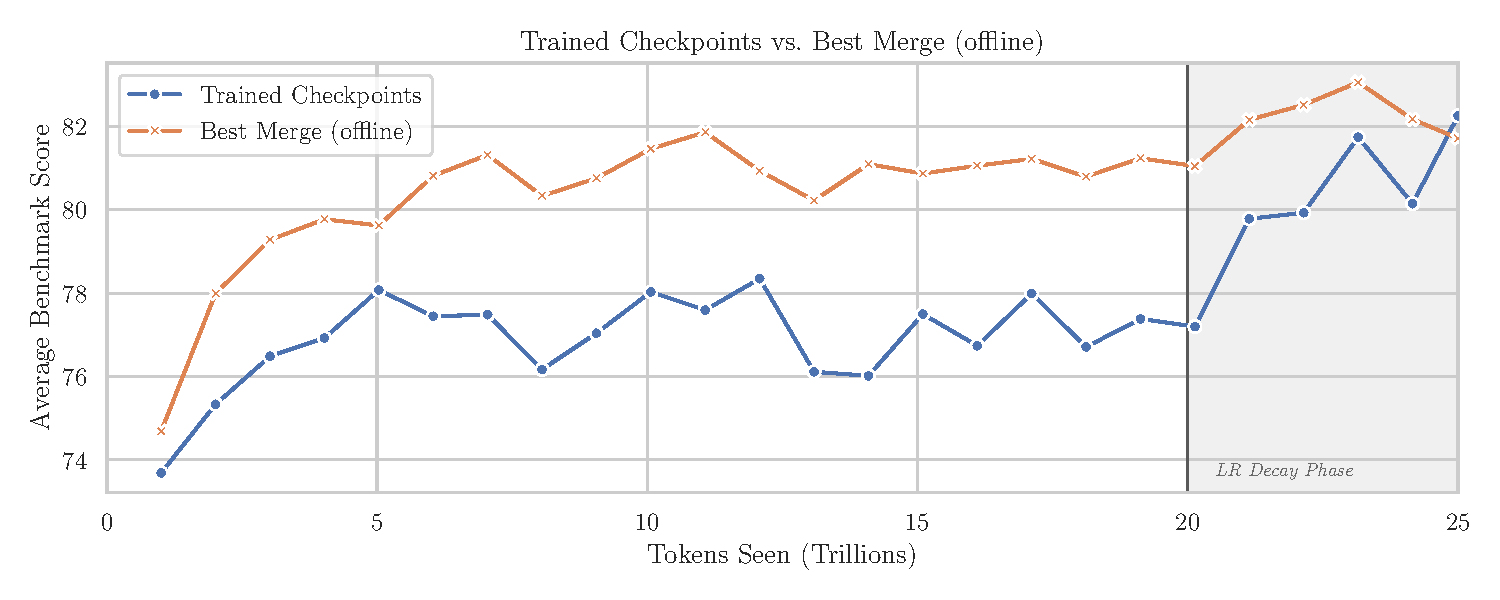
\includegraphics[width=0.9\textwidth]{figures/avg_benchmark.pdf}
    \caption{Average accuracy across 12 benchmarks for trained checkpoints versus the best offline checkpoint merge during pretraining. During the stable LR phase, offline merging yields a consistent 2--4 point improvement. During the LR decay phase (shaded), the gap narrows as trained checkpoints benefit from actual learning rate annealing.}
    \label{fig:avg-benchmark}
\end{figure}

During the final 5T-token LR decay phase (from 20T to 25T tokens), the gap between merged and trained checkpoints narrows substantially, and the two evaluation trajectories largely coincide by the end of training. \citet{tian2025wsm} reported that combining merging with decay offers no gain over merging alone, so this convergence is expected. The original WSM results went further, showing merge-based readouts \emph{surpassing} decay-trained checkpoints. In experiments on the Nemotron 3 Nano scale architecture (30B-A3B), we were able to reproduce such gains when emulating short (${\sim}500$B) decay windows. However, direct comparisons at 1T and 1.5T merge horizons showed no improvement over decay-trained checkpoints.

Our takeaway is that offline checkpoint merging appears most effective for shorter annealing horizons. This is consistent with~\citet{ling2025foundation}, who employ a comparably short decay schedule and report merge-based improvements, in contrast with the much longer 5T decay used here, where trained decay is able to match or surpass merge-based readouts. The final base model checkpoint selected for downstream alignment was itself a 500B merge; short-horizon merging remains practically useful even alongside a full decay schedule. That said, our experiments explored only a single merge schedule (\texttt{minus-sqrt}) and a fixed checkpoint granularity; it remains plausible that alternative coefficient schemes, finer-grained checkpoint windows, or merging strategies tailored to longer decay horizons could recover the gains observed at shorter scales. Per-benchmark breakdowns are provided in Appendix Figure~\ref{fig:per-benchmark}.

\subsection{Long-Context Extension}\label{sec:pre-train-long-context}

Similar to Nemotron 3 Nano, we added a long-context phase (LC-Phase) at the end of pretraining. In the LC-Phase, we performed continuous pretraining (CPT) to equip the base model with long-context ability. We used a constant learning rate of $4.5*10^{-6}$ and global batch size of 16. We used 64-way context parallelism, 2-way tensor parallelism, and 64-way expert parallelism to train on GB200 GPUs. We reused the long-context document QA dataset from Nemotron 2 \& 3 Nano. We allocated the document QA data to 20\% in the Phase LC data blend, with the remaining 80\% being downscaled Phase 2 data. We initially performed CPT on 1,048,576 (1m) context length. Such stage lasted for 34 billion tokens. Following that we added another stage to alternatingly train on both 1m and 4k sequences in order to mitigate the minor impact we observed on the math-related benchmarks. The second stage lasted for 17 billion tokens.

